\documentclass[1p]{elsarticle_modified}
%\bibliographystyle{elsarticle-num}

%\usepackage[colorlinks]{hyperref}
%\usepackage{abbrmath_seonhwa} %\Abb, \Ascr, \Acal ,\Abf, \Afrak
\usepackage{amsfonts}
\usepackage{amssymb}
\usepackage{amsmath}
\usepackage{amsthm}
\usepackage{scalefnt}
\usepackage{amsbsy}
\usepackage{kotex}
\usepackage{caption}
\usepackage{subfig}
\usepackage{color}
\usepackage{graphicx}
\usepackage{xcolor} %% white, black, red, green, blue, cyan, magenta, yellow
\usepackage{float}
\usepackage{setspace}
\usepackage{hyperref}

\usepackage{tikz}
\usetikzlibrary{arrows}

\usepackage{multirow}
\usepackage{array} % fixed length table
\usepackage{hhline}

%%%%%%%%%%%%%%%%%%%%%
\makeatletter
\renewcommand*\env@matrix[1][\arraystretch]{%
	\edef\arraystretch{#1}%
	\hskip -\arraycolsep
	\let\@ifnextchar\new@ifnextchar
	\array{*\c@MaxMatrixCols c}}
\makeatother %https://tex.stackexchange.com/questions/14071/how-can-i-increase-the-line-spacing-in-a-matrix
%%%%%%%%%%%%%%%

\usepackage[normalem]{ulem}

\newcommand{\msout}[1]{\ifmmode\text{\sout{\ensuremath{#1}}}\else\sout{#1}\fi}
%SOURCE: \msout is \stkout macro in https://tex.stackexchange.com/questions/20609/strikeout-in-math-mode

\newcommand{\cancel}[1]{
	\ifmmode
	{\color{red}\msout{#1}}
	\else
	{\color{red}\sout{#1}}
	\fi
}

\newcommand{\add}[1]{
	{\color{blue}\uwave{#1}}
}

\newcommand{\replace}[2]{
	\ifmmode
	{\color{red}\msout{#1}}{\color{blue}\uwave{#2}}
	\else
	{\color{red}\sout{#1}}{\color{blue}\uwave{#2}}
	\fi
}

\newcommand{\Sol}{\mathcal{S}} %segment
\newcommand{\D}{D} %diagram
\newcommand{\A}{\mathcal{A}} %arc


%%%%%%%%%%%%%%%%%%%%%%%%%%%%%5 test

\def\sl{\operatorname{\textup{SL}}(2,\Cbb)}
\def\psl{\operatorname{\textup{PSL}}(2,\Cbb)}
\def\quan{\mkern 1mu \triangleright \mkern 1mu}

\theoremstyle{definition}
\newtheorem{thm}{Theorem}[section]
\newtheorem{prop}[thm]{Proposition}
\newtheorem{lem}[thm]{Lemma}
\newtheorem{ques}[thm]{Question}
\newtheorem{cor}[thm]{Corollary}
\newtheorem{defn}[thm]{Definition}
\newtheorem{exam}[thm]{Example}
\newtheorem{rmk}[thm]{Remark}
\newtheorem{alg}[thm]{Algorithm}

\newcommand{\I}{\sqrt{-1}}
\begin{document}

%\begin{frontmatter}
%
%\title{Boundary parabolic representations of knots up to 8 crossings}
%
%%% Group authors per affiliation:
%\author{Yunhi Cho} 
%\address{Department of Mathematics, University of Seoul, Seoul, Korea}
%\ead{yhcho@uos.ac.kr}
%
%
%\author{Seonhwa Kim} %\fnref{s_kim}}
%\address{Center for Geometry and Physics, Institute for Basic Science, Pohang, 37673, Korea}
%\ead{ryeona17@ibs.re.kr}
%
%\author{Hyuk Kim}
%\address{Department of Mathematical Sciences, Seoul National University, Seoul 08826, Korea}
%\ead{hyukkim@snu.ac.kr}
%
%\author{Seokbeom Yoon}
%\address{Department of Mathematical Sciences, Seoul National University, Seoul, 08826,  Korea}
%\ead{sbyoon15@snu.ac.kr}
%
%\begin{abstract}
%We find all boundary parabolic representation of knots up to 8 crossings.
%
%\end{abstract}
%\begin{keyword}
%    \MSC[2010] 57M25 
%\end{keyword}
%
%\end{frontmatter}

%\linenumbers
%\tableofcontents
%
\newcommand\colored[1]{\textcolor{white}{\rule[-0.35ex]{0.8em}{1.4ex}}\kern-0.8em\color{red} #1}%
%\newcommand\colored[1]{\textcolor{white}{ #1}\kern-2.17ex	\textcolor{white}{ #1}\kern-1.81ex	\textcolor{white}{ #1}\kern-2.15ex\color{red}#1	}

{\Large $\underline{12a_{0143}~(K12a_{0143})}$}

\setlength{\tabcolsep}{10pt}
\renewcommand{\arraystretch}{1.6}
\vspace{1cm}\begin{tabular}{m{100pt}>{\centering\arraybackslash}m{274pt}}
\multirow{5}{120pt}{
	\centering
	\includegraphics[width=112pt]{../../../GIT/diagram.site/Diagrams/png/944_12a_0143.png}\\
\ \ \ A knot diagram\footnotemark}&
\allowdisplaybreaks
\textbf{Linearized knot diagam} \\
\cline{2-2}
 &
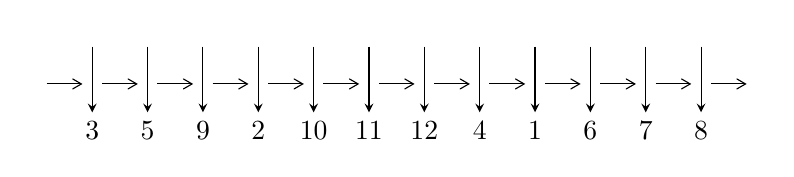
\begin{tikzpicture}[x=20pt, y=17pt]
	% nodes
	\node (C0) at (0, 0) {};
	\node (C1) at (1, 0) {};
	\node (C1U) at (1, +1) {};
	\node (C1D) at (1, -1) {3};

	\node (C2) at (2, 0) {};
	\node (C2U) at (2, +1) {};
	\node (C2D) at (2, -1) {5};

	\node (C3) at (3, 0) {};
	\node (C3U) at (3, +1) {};
	\node (C3D) at (3, -1) {9};

	\node (C4) at (4, 0) {};
	\node (C4U) at (4, +1) {};
	\node (C4D) at (4, -1) {2};

	\node (C5) at (5, 0) {};
	\node (C5U) at (5, +1) {};
	\node (C5D) at (5, -1) {10};

	\node (C6) at (6, 0) {};
	\node (C6U) at (6, +1) {};
	\node (C6D) at (6, -1) {11};

	\node (C7) at (7, 0) {};
	\node (C7U) at (7, +1) {};
	\node (C7D) at (7, -1) {12};

	\node (C8) at (8, 0) {};
	\node (C8U) at (8, +1) {};
	\node (C8D) at (8, -1) {4};

	\node (C9) at (9, 0) {};
	\node (C9U) at (9, +1) {};
	\node (C9D) at (9, -1) {1};

	\node (C10) at (10, 0) {};
	\node (C10U) at (10, +1) {};
	\node (C10D) at (10, -1) {6};

	\node (C11) at (11, 0) {};
	\node (C11U) at (11, +1) {};
	\node (C11D) at (11, -1) {7};

	\node (C12) at (12, 0) {};
	\node (C12U) at (12, +1) {};
	\node (C12D) at (12, -1) {8};
	\node (C13) at (13, 0) {};

	% arrows
	\draw[->,>={angle 60}]
	(C0) edge (C1) (C1) edge (C2) (C2) edge (C3) (C3) edge (C4) (C4) edge (C5) (C5) edge (C6) (C6) edge (C7) (C7) edge (C8) (C8) edge (C9) (C9) edge (C10) (C10) edge (C11) (C11) edge (C12) (C12) edge (C13) ;	\draw[->,>=stealth]
	(C1U) edge (C1D) (C2U) edge (C2D) (C3U) edge (C3D) (C4U) edge (C4D) (C5U) edge (C5D) (C6U) edge (C6D) (C7U) edge (C7D) (C8U) edge (C8D) (C9U) edge (C9D) (C10U) edge (C10D) (C11U) edge (C11D) (C12U) edge (C12D) ;
	\end{tikzpicture} \\
\hhline{~~} \\& 
\textbf{Solving Sequence} \\ \cline{2-2} 
 &
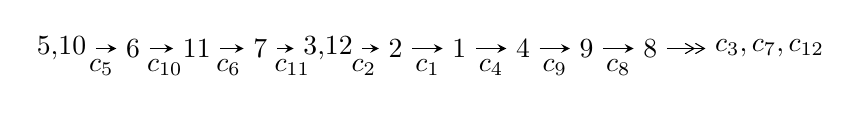
\begin{tikzpicture}[x=23pt, y=7pt]
	% node
	\node (A0) at (-1/8, 0) {5,10};
	\node (A1) at (1, 0) {6};
	\node (A2) at (2, 0) {11};
	\node (A3) at (3, 0) {7};
	\node (A4) at (65/16, 0) {3,12};
	\node (A5) at (41/8, 0) {2};
	\node (A6) at (49/8, 0) {1};
	\node (A7) at (57/8, 0) {4};
	\node (A8) at (65/8, 0) {9};
	\node (A9) at (73/8, 0) {8};
	\node (C1) at (1/2, -1) {$c_{5}$};
	\node (C2) at (3/2, -1) {$c_{10}$};
	\node (C3) at (5/2, -1) {$c_{6}$};
	\node (C4) at (7/2, -1) {$c_{11}$};
	\node (C5) at (37/8, -1) {$c_{2}$};
	\node (C6) at (45/8, -1) {$c_{1}$};
	\node (C7) at (53/8, -1) {$c_{4}$};
	\node (C8) at (61/8, -1) {$c_{9}$};
	\node (C9) at (69/8, -1) {$c_{8}$};
	\node (A10) at (11, 0) {$c_{3},c_{7},c_{12}$};

	% edge
	\draw[->,>=stealth]	
	(A0) edge (A1) (A1) edge (A2) (A2) edge (A3) (A3) edge (A4) (A4) edge (A5) (A5) edge (A6) (A6) edge (A7) (A7) edge (A8) (A8) edge (A9) ;
	\draw[->>,>={angle 60}]	
	(A9) edge (A10);
\end{tikzpicture} \\ 

\end{tabular} \\

\footnotetext{
The image of knot diagram is generated by the software ``\textbf{Draw programme}" developed by Andrew Bartholomew(\url{http://www.layer8.co.uk/maths/draw/index.htm\#Running-draw}), where we modified some parts for our purpose(\url{https://github.com/CATsTAILs/LinksPainter}).
}\phantom \\ \newline 
\centering \textbf{Ideals for irreducible components\footnotemark of $X_{\text{par}}$} 
 
\begin{align*}
I^u_{1}&=\langle 
- u^{44}- u^{43}+\cdots+b+1,\;- u^{26}+19 u^{24}+\cdots+a-1,\;u^{45}+2 u^{44}+\cdots+u-1\rangle \\
I^u_{2}&=\langle 
b+1,\;a+1,\;u^3- u^2-2 u+1\rangle \\
\\
\end{align*}
\raggedright * 2 irreducible components of $\dim_{\mathbb{C}}=0$, with total 48 representations.\\
\footnotetext{All coefficients of polynomials are rational numbers. But the coefficients are sometimes approximated in decimal forms when there is not enough margin.}
\newpage
\renewcommand{\arraystretch}{1}
\centering \section*{I. $I^u_{1}= \langle - u^{44}- u^{43}+\cdots+b+1,\;- u^{26}+19 u^{24}+\cdots+a-1,\;u^{45}+2 u^{44}+\cdots+u-1 \rangle$}
\flushleft \textbf{(i) Arc colorings}\\
\begin{tabular}{m{7pt} m{180pt} m{7pt} m{180pt} }
\flushright $a_{5}=$&$\begin{pmatrix}1\\0\end{pmatrix}$ \\
\flushright $a_{10}=$&$\begin{pmatrix}0\\u\end{pmatrix}$ \\
\flushright $a_{6}=$&$\begin{pmatrix}1\\u^2\end{pmatrix}$ \\
\flushright $a_{11}=$&$\begin{pmatrix}- u\\- u^3+u\end{pmatrix}$ \\
\flushright $a_{7}=$&$\begin{pmatrix}- u^2+1\\- u^4+2 u^2\end{pmatrix}$ \\
\flushright $a_{3}=$&$\begin{pmatrix}u^{26}-19 u^{24}+\cdots+2 u+1\\u^{44}+u^{43}+\cdots+u-1\end{pmatrix}$ \\
\flushright $a_{12}=$&$\begin{pmatrix}u^3-2 u\\u^5-3 u^3+u\end{pmatrix}$ \\
\flushright $a_{2}=$&$\begin{pmatrix}u^{44}+u^{43}+\cdots-19 u^3+3 u\\u^{44}+u^{43}+\cdots+u-1\end{pmatrix}$ \\
\flushright $a_{1}=$&$\begin{pmatrix}u^5-4 u^3+3 u\\u^7-5 u^5+6 u^3- u\end{pmatrix}$ \\
\flushright $a_{4}=$&$\begin{pmatrix}2 u^{44}+2 u^{43}+\cdots+4 u^2+3 u\\u^{44}+u^{43}+\cdots+2 u-1\end{pmatrix}$ \\
\flushright $a_{9}=$&$\begin{pmatrix}u^{11}-8 u^9+22 u^7-24 u^5+9 u^3\\u^{13}-9 u^{11}+29 u^9-40 u^7+22 u^5-3 u^3+u\end{pmatrix}$ \\
\flushright $a_{8}=$&$\begin{pmatrix}u^4-3 u^2+1\\u^6-4 u^4+3 u^2\end{pmatrix}$\\&\end{tabular}
\flushleft \textbf{(ii) Obstruction class $= -1$}\\~\\
\flushleft \textbf{(iii) Cusp Shapes $= 5 u^{44}+4 u^{43}+\cdots-4 u-19$}\\~\\
\newpage\renewcommand{\arraystretch}{1}
\flushleft \textbf{(iv) u-Polynomials at the component}\newline \\
\begin{tabular}{m{50pt}|m{274pt}}
Crossings & \hspace{64pt}u-Polynomials at each crossing \\
\hline $$\begin{aligned}c_{1}\end{aligned}$$&$\begin{aligned}
&u^{45}+22 u^{44}+\cdots+74 u+1
\end{aligned}$\\
\hline $$\begin{aligned}c_{2},c_{4}\end{aligned}$$&$\begin{aligned}
&u^{45}-4 u^{44}+\cdots+6 u+1
\end{aligned}$\\
\hline $$\begin{aligned}c_{3},c_{8}\end{aligned}$$&$\begin{aligned}
&u^{45}- u^{44}+\cdots+12 u+8
\end{aligned}$\\
\hline $$\begin{aligned}c_{5},c_{6},c_{7}\\c_{10},c_{11},c_{12}\end{aligned}$$&$\begin{aligned}
&u^{45}-2 u^{44}+\cdots+u+1
\end{aligned}$\\
\hline $$\begin{aligned}c_{9}\end{aligned}$$&$\begin{aligned}
&u^{45}+8 u^{44}+\cdots+409 u+55
\end{aligned}$\\
\hline
\end{tabular}\\~\\
\newpage\renewcommand{\arraystretch}{1}
\flushleft \textbf{(v) Riley Polynomials at the component}\newline \\
\begin{tabular}{m{50pt}|m{274pt}}
Crossings & \hspace{64pt}Riley Polynomials at each crossing \\
\hline $$\begin{aligned}c_{1}\end{aligned}$$&$\begin{aligned}
&y^{45}+6 y^{44}+\cdots+4358 y-1
\end{aligned}$\\
\hline $$\begin{aligned}c_{2},c_{4}\end{aligned}$$&$\begin{aligned}
&y^{45}-22 y^{44}+\cdots+74 y-1
\end{aligned}$\\
\hline $$\begin{aligned}c_{3},c_{8}\end{aligned}$$&$\begin{aligned}
&y^{45}+21 y^{44}+\cdots+16 y-64
\end{aligned}$\\
\hline $$\begin{aligned}c_{5},c_{6},c_{7}\\c_{10},c_{11},c_{12}\end{aligned}$$&$\begin{aligned}
&y^{45}-64 y^{44}+\cdots+13 y-1
\end{aligned}$\\
\hline $$\begin{aligned}c_{9}\end{aligned}$$&$\begin{aligned}
&y^{45}-4 y^{44}+\cdots-43479 y-3025
\end{aligned}$\\
\hline
\end{tabular}\\~\\
\newpage\flushleft \textbf{(vi) Complex Volumes and Cusp Shapes}
$$\begin{array}{c|c|c}  
\text{Solutions to }I^u_{1}& \I (\text{vol} + \sqrt{-1}CS) & \text{Cusp shape}\\
 \hline 
\begin{aligned}
u &= \phantom{-}0.962969 + 0.169603 I \\
a &= \phantom{-}0.440533 - 0.958645 I \\
b &= \phantom{-}0.692370 + 0.677447 I\end{aligned}
 & -0.28984 - 2.31607 I & -13.48731 + 4.06907 I \\ \hline\begin{aligned}
u &= \phantom{-}0.962969 - 0.169603 I \\
a &= \phantom{-}0.440533 + 0.958645 I \\
b &= \phantom{-}0.692370 - 0.677447 I\end{aligned}
 & -0.28984 + 2.31607 I & -13.48731 - 4.06907 I \\ \hline\begin{aligned}
u &= -1.148590 + 0.071392 I \\
a &= \phantom{-}0.801348 + 0.494679 I \\
b &= -0.427212 - 0.486489 I\end{aligned}
 & -5.22276 + 0.37204 I & \phantom{-0.000000 } 0 \\ \hline\begin{aligned}
u &= -1.148590 - 0.071392 I \\
a &= \phantom{-}0.801348 - 0.494679 I \\
b &= -0.427212 + 0.486489 I\end{aligned}
 & -5.22276 - 0.37204 I & \phantom{-0.000000 } 0 \\ \hline\begin{aligned}
u &= \phantom{-}1.176560 + 0.211087 I \\
a &= -0.653062 + 0.188078 I \\
b &= \phantom{-}0.348834 - 0.855887 I\end{aligned}
 & -2.36170 - 5.17327 I & \phantom{-0.000000 } 0 \\ \hline\begin{aligned}
u &= \phantom{-}1.176560 - 0.211087 I \\
a &= -0.653062 - 0.188078 I \\
b &= \phantom{-}0.348834 + 0.855887 I\end{aligned}
 & -2.36170 + 5.17327 I & \phantom{-0.000000 } 0 \\ \hline\begin{aligned}
u &= \phantom{-}0.763709 + 0.251528 I \\
a &= -0.0103561 - 0.1259090 I \\
b &= \phantom{-}0.955005 - 0.546675 I\end{aligned}
 & -1.03136 + 2.41021 I & -15.6897 - 1.6774 I \\ \hline\begin{aligned}
u &= \phantom{-}0.763709 - 0.251528 I \\
a &= -0.0103561 + 0.1259090 I \\
b &= \phantom{-}0.955005 + 0.546675 I\end{aligned}
 & -1.03136 - 2.41021 I & -15.6897 + 1.6774 I \\ \hline\begin{aligned}
u &= \phantom{-}1.191250 + 0.124036 I \\
a &= -1.094580 + 0.310585 I \\
b &= -1.252440 + 0.198803 I\end{aligned}
 & -7.65311 - 1.99196 I & \phantom{-0.000000 } 0 \\ \hline\begin{aligned}
u &= \phantom{-}1.191250 - 0.124036 I \\
a &= -1.094580 - 0.310585 I \\
b &= -1.252440 - 0.198803 I\end{aligned}
 & -7.65311 + 1.99196 I & \phantom{-0.000000 } 0\\
 \hline 
 \end{array}$$\newpage$$\begin{array}{c|c|c}  
\text{Solutions to }I^u_{1}& \I (\text{vol} + \sqrt{-1}CS) & \text{Cusp shape}\\
 \hline 
\begin{aligned}
u &= -1.191140 + 0.163730 I \\
a &= -0.78548 - 1.96254 I \\
b &= -1.029290 + 0.504098 I\end{aligned}
 & -6.91071 + 4.51785 I & \phantom{-0.000000 } 0 \\ \hline\begin{aligned}
u &= -1.191140 - 0.163730 I \\
a &= -0.78548 + 1.96254 I \\
b &= -1.029290 - 0.504098 I\end{aligned}
 & -6.91071 - 4.51785 I & \phantom{-0.000000 } 0 \\ \hline\begin{aligned}
u &= \phantom{-}1.219810 + 0.229016 I \\
a &= \phantom{-}1.09073 - 1.61980 I \\
b &= \phantom{-}1.150280 + 0.609142 I\end{aligned}
 & -4.75327 - 10.58690 I & \phantom{-0.000000 } 0 \\ \hline\begin{aligned}
u &= \phantom{-}1.219810 - 0.229016 I \\
a &= \phantom{-}1.09073 + 1.61980 I \\
b &= \phantom{-}1.150280 - 0.609142 I\end{aligned}
 & -4.75327 + 10.58690 I & \phantom{-0.000000 } 0 \\ \hline\begin{aligned}
u &= -1.316520 + 0.069582 I \\
a &= \phantom{-}0.845369 + 0.138843 I \\
b &= \phantom{-}0.949980 + 0.382113 I\end{aligned}
 & -7.86567 - 1.43041 I & \phantom{-0.000000 } 0 \\ \hline\begin{aligned}
u &= -1.316520 - 0.069582 I \\
a &= \phantom{-}0.845369 - 0.138843 I \\
b &= \phantom{-}0.949980 - 0.382113 I\end{aligned}
 & -7.86567 + 1.43041 I & \phantom{-0.000000 } 0 \\ \hline\begin{aligned}
u &= -0.503453 + 0.459470 I \\
a &= \phantom{-}0.37795 + 2.46430 I \\
b &= \phantom{-}1.101250 - 0.610224 I\end{aligned}
 & \phantom{-}0.78058 + 8.20264 I & -13.8836 - 9.3349 I \\ \hline\begin{aligned}
u &= -0.503453 - 0.459470 I \\
a &= \phantom{-}0.37795 - 2.46430 I \\
b &= \phantom{-}1.101250 + 0.610224 I\end{aligned}
 & \phantom{-}0.78058 - 8.20264 I & -13.8836 + 9.3349 I \\ \hline\begin{aligned}
u &= -0.432497 + 0.443637 I \\
a &= -1.29853 - 0.73079 I \\
b &= \phantom{-}0.428503 + 0.789342 I\end{aligned}
 & \phantom{-}2.77707 + 2.93987 I & -10.12479 - 5.18879 I \\ \hline\begin{aligned}
u &= -0.432497 - 0.443637 I \\
a &= -1.29853 + 0.73079 I \\
b &= \phantom{-}0.428503 - 0.789342 I\end{aligned}
 & \phantom{-}2.77707 - 2.93987 I & -10.12479 + 5.18879 I\\
 \hline 
 \end{array}$$\newpage$$\begin{array}{c|c|c}  
\text{Solutions to }I^u_{1}& \I (\text{vol} + \sqrt{-1}CS) & \text{Cusp shape}\\
 \hline 
\begin{aligned}
u &= \phantom{-}0.442889 + 0.349610 I \\
a &= \phantom{-}0.03028 + 3.06490 I \\
b &= -0.954541 - 0.430846 I\end{aligned}
 & -1.64546 - 2.76575 I & -16.0685 + 7.3874 I \\ \hline\begin{aligned}
u &= \phantom{-}0.442889 - 0.349610 I \\
a &= \phantom{-}0.03028 - 3.06490 I \\
b &= -0.954541 + 0.430846 I\end{aligned}
 & -1.64546 + 2.76575 I & -16.0685 - 7.3874 I \\ \hline\begin{aligned}
u &= -0.147862 + 0.512639 I \\
a &= -1.34459 - 1.27617 I \\
b &= \phantom{-}1.043660 + 0.604880 I\end{aligned}
 & \phantom{-}1.83508 - 4.99628 I & -10.28872 + 3.31837 I \\ \hline\begin{aligned}
u &= -0.147862 - 0.512639 I \\
a &= -1.34459 + 1.27617 I \\
b &= \phantom{-}1.043660 - 0.604880 I\end{aligned}
 & \phantom{-}1.83508 + 4.99628 I & -10.28872 - 3.31837 I \\ \hline\begin{aligned}
u &= -0.229805 + 0.471597 I \\
a &= -0.25152 + 1.93643 I \\
b &= \phantom{-}0.527284 - 0.732325 I\end{aligned}
 & \phantom{-}3.37526 + 0.10760 I & -7.61315 - 2.95177 I \\ \hline\begin{aligned}
u &= -0.229805 - 0.471597 I \\
a &= -0.25152 - 1.93643 I \\
b &= \phantom{-}0.527284 + 0.732325 I\end{aligned}
 & \phantom{-}3.37526 - 0.10760 I & -7.61315 + 2.95177 I \\ \hline\begin{aligned}
u &= -0.426938 + 0.242547 I \\
a &= -0.516634 - 0.830332 I \\
b &= -1.145690 - 0.133170 I\end{aligned}
 & -2.39909 + 0.70824 I & -15.1495 - 9.1471 I \\ \hline\begin{aligned}
u &= -0.426938 - 0.242547 I \\
a &= -0.516634 + 0.830332 I \\
b &= -1.145690 + 0.133170 I\end{aligned}
 & -2.39909 - 0.70824 I & -15.1495 + 9.1471 I \\ \hline\begin{aligned}
u &= \phantom{-}0.181432 + 0.311155 I \\
a &= \phantom{-}2.35597 - 1.25070 I \\
b &= -0.825100 + 0.293052 I\end{aligned}
 & -0.905303 + 0.433735 I & -12.18552 + 1.89292 I \\ \hline\begin{aligned}
u &= \phantom{-}0.181432 - 0.311155 I \\
a &= \phantom{-}2.35597 + 1.25070 I \\
b &= -0.825100 - 0.293052 I\end{aligned}
 & -0.905303 - 0.433735 I & -12.18552 - 1.89292 I\\
 \hline 
 \end{array}$$\newpage$$\begin{array}{c|c|c}  
\text{Solutions to }I^u_{1}& \I (\text{vol} + \sqrt{-1}CS) & \text{Cusp shape}\\
 \hline 
\begin{aligned}
u &= \phantom{-}0.346739\phantom{ +0.000000I} \\
a &= \phantom{-}1.01677\phantom{ +0.000000I} \\
b &= -0.122928\phantom{ +0.000000I}\end{aligned}
 & -0.548092\phantom{ +0.000000I} & -17.9540\phantom{ +0.000000I} \\ \hline\begin{aligned}
u &= -1.73488 + 0.01556 I \\
a &= \phantom{-}0.165858 + 0.798942 I \\
b &= \phantom{-}0.805113 - 0.767877 I\end{aligned}
 & -10.02540 + 2.83788 I & \phantom{-0.000000 } 0 \\ \hline\begin{aligned}
u &= -1.73488 - 0.01556 I \\
a &= \phantom{-}0.165858 - 0.798942 I \\
b &= \phantom{-}0.805113 + 0.767877 I\end{aligned}
 & -10.02540 - 2.83788 I & \phantom{-0.000000 } 0 \\ \hline\begin{aligned}
u &= \phantom{-}1.77511 + 0.02023 I \\
a &= \phantom{-}0.581848 - 0.527304 I \\
b &= -0.425874 + 0.628346 I\end{aligned}
 & -15.9251 - 0.7872 I & \phantom{-0.000000 } 0 \\ \hline\begin{aligned}
u &= \phantom{-}1.77511 - 0.02023 I \\
a &= \phantom{-}0.581848 + 0.527304 I \\
b &= -0.425874 - 0.628346 I\end{aligned}
 & -15.9251 + 0.7872 I & \phantom{-0.000000 } 0 \\ \hline\begin{aligned}
u &= -1.77793 + 0.05224 I \\
a &= -0.414828 - 0.211707 I \\
b &= \phantom{-}0.314583 + 0.909747 I\end{aligned}
 & -13.1145 + 6.3153 I & \phantom{-0.000000 } 0 \\ \hline\begin{aligned}
u &= -1.77793 - 0.05224 I \\
a &= -0.414828 + 0.211707 I \\
b &= \phantom{-}0.314583 - 0.909747 I\end{aligned}
 & -13.1145 - 6.3153 I & \phantom{-0.000000 } 0 \\ \hline\begin{aligned}
u &= \phantom{-}1.78253 + 0.04085 I \\
a &= -0.78346 + 1.57093 I \\
b &= -1.063730 - 0.545729 I\end{aligned}
 & -17.7770 - 5.4165 I & \phantom{-0.000000 } 0 \\ \hline\begin{aligned}
u &= \phantom{-}1.78253 - 0.04085 I \\
a &= -0.78346 - 1.57093 I \\
b &= -1.063730 + 0.545729 I\end{aligned}
 & -17.7770 + 5.4165 I & \phantom{-0.000000 } 0 \\ \hline\begin{aligned}
u &= -1.78292 + 0.03166 I \\
a &= -1.096720 - 0.115819 I \\
b &= -1.302410 - 0.221345 I\end{aligned}
 & -18.5397 + 2.6826 I & \phantom{-0.000000 } 0\\
 \hline 
 \end{array}$$\newpage$$\begin{array}{c|c|c}  
\text{Solutions to }I^u_{1}& \I (\text{vol} + \sqrt{-1}CS) & \text{Cusp shape}\\
 \hline 
\begin{aligned}
u &= -1.78292 - 0.03166 I \\
a &= -1.096720 + 0.115819 I \\
b &= -1.302410 + 0.221345 I\end{aligned}
 & -18.5397 - 2.6826 I & \phantom{-0.000000 } 0 \\ \hline\begin{aligned}
u &= -1.78906 + 0.05870 I \\
a &= \phantom{-}1.08096 + 1.26242 I \\
b &= \phantom{-}1.181650 - 0.611600 I\end{aligned}
 & -15.7314 + 11.8740 I & \phantom{-0.000000 } 0 \\ \hline\begin{aligned}
u &= -1.78906 - 0.05870 I \\
a &= \phantom{-}1.08096 - 1.26242 I \\
b &= \phantom{-}1.181650 + 0.611600 I\end{aligned}
 & -15.7314 - 11.8740 I & \phantom{-0.000000 } 0 \\ \hline\begin{aligned}
u &= \phantom{-}1.81198 + 0.01590 I \\
a &= \phantom{-}0.970531 - 0.091202 I \\
b &= \phantom{-}0.989237 - 0.314096 I\end{aligned}
 & -19.4518 + 1.0384 I & \phantom{-0.000000 } 0 \\ \hline\begin{aligned}
u &= \phantom{-}1.81198 - 0.01590 I \\
a &= \phantom{-}0.970531 + 0.091202 I \\
b &= \phantom{-}0.989237 + 0.314096 I\end{aligned}
 & -19.4518 - 1.0384 I & \phantom{-0.000000 } 0\\
 \hline 
 \end{array}$$\newpage\newpage\renewcommand{\arraystretch}{1}
\centering \section*{II. $I^u_{2}= \langle b+1,\;a+1,\;u^3- u^2-2 u+1 \rangle$}
\flushleft \textbf{(i) Arc colorings}\\
\begin{tabular}{m{7pt} m{180pt} m{7pt} m{180pt} }
\flushright $a_{5}=$&$\begin{pmatrix}1\\0\end{pmatrix}$ \\
\flushright $a_{10}=$&$\begin{pmatrix}0\\u\end{pmatrix}$ \\
\flushright $a_{6}=$&$\begin{pmatrix}1\\u^2\end{pmatrix}$ \\
\flushright $a_{11}=$&$\begin{pmatrix}- u\\- u^2- u+1\end{pmatrix}$ \\
\flushright $a_{7}=$&$\begin{pmatrix}- u^2+1\\- u^2- u+1\end{pmatrix}$ \\
\flushright $a_{3}=$&$\begin{pmatrix}-1\\-1\end{pmatrix}$ \\
\flushright $a_{12}=$&$\begin{pmatrix}u^2-1\\u^2\end{pmatrix}$ \\
\flushright $a_{2}=$&$\begin{pmatrix}-2\\-1\end{pmatrix}$ \\
\flushright $a_{1}=$&$\begin{pmatrix}-1\\0\end{pmatrix}$ \\
\flushright $a_{4}=$&$\begin{pmatrix}-1\\-1\end{pmatrix}$ \\
\flushright $a_{9}=$&$\begin{pmatrix}u\\u\end{pmatrix}$ \\
\flushright $a_{8}=$&$\begin{pmatrix}u\\u\end{pmatrix}$\\&\end{tabular}
\flushleft \textbf{(ii) Obstruction class $= 1$}\\~\\
\flushleft \textbf{(iii) Cusp Shapes $= - u^2+u-17$}\\~\\
\newpage\renewcommand{\arraystretch}{1}
\flushleft \textbf{(iv) u-Polynomials at the component}\newline \\
\begin{tabular}{m{50pt}|m{274pt}}
Crossings & \hspace{64pt}u-Polynomials at each crossing \\
\hline $$\begin{aligned}c_{1},c_{2}\end{aligned}$$&$\begin{aligned}
&(u-1)^3
\end{aligned}$\\
\hline $$\begin{aligned}c_{3},c_{8}\end{aligned}$$&$\begin{aligned}
&u^3
\end{aligned}$\\
\hline $$\begin{aligned}c_{4}\end{aligned}$$&$\begin{aligned}
&(u+1)^3
\end{aligned}$\\
\hline $$\begin{aligned}c_{5},c_{6},c_{7}\\c_{9}\end{aligned}$$&$\begin{aligned}
&u^3- u^2-2 u+1
\end{aligned}$\\
\hline $$\begin{aligned}c_{10},c_{11},c_{12}\end{aligned}$$&$\begin{aligned}
&u^3+u^2-2 u-1
\end{aligned}$\\
\hline
\end{tabular}\\~\\
\newpage\renewcommand{\arraystretch}{1}
\flushleft \textbf{(v) Riley Polynomials at the component}\newline \\
\begin{tabular}{m{50pt}|m{274pt}}
Crossings & \hspace{64pt}Riley Polynomials at each crossing \\
\hline $$\begin{aligned}c_{1},c_{2},c_{4}\end{aligned}$$&$\begin{aligned}
&(y-1)^3
\end{aligned}$\\
\hline $$\begin{aligned}c_{3},c_{8}\end{aligned}$$&$\begin{aligned}
&y^3
\end{aligned}$\\
\hline $$\begin{aligned}c_{5},c_{6},c_{7}\\c_{9},c_{10},c_{11}\\c_{12}\end{aligned}$$&$\begin{aligned}
&y^3-5 y^2+6 y-1
\end{aligned}$\\
\hline
\end{tabular}\\~\\
\newpage\flushleft \textbf{(vi) Complex Volumes and Cusp Shapes}
$$\begin{array}{c|c|c}  
\text{Solutions to }I^u_{2}& \I (\text{vol} + \sqrt{-1}CS) & \text{Cusp shape}\\
 \hline 
\begin{aligned}
u &= -1.24698\phantom{ +0.000000I} \\
a &= -1.00000\phantom{ +0.000000I} \\
b &= -1.00000\phantom{ +0.000000I}\end{aligned}
 & -7.98968\phantom{ +0.000000I} & -19.8020\phantom{ +0.000000I} \\ \hline\begin{aligned}
u &= \phantom{-}0.445042\phantom{ +0.000000I} \\
a &= -1.00000\phantom{ +0.000000I} \\
b &= -1.00000\phantom{ +0.000000I}\end{aligned}
 & -2.34991\phantom{ +0.000000I} & -16.7530\phantom{ +0.000000I} \\ \hline\begin{aligned}
u &= \phantom{-}1.80194\phantom{ +0.000000I} \\
a &= -1.00000\phantom{ +0.000000I} \\
b &= -1.00000\phantom{ +0.000000I}\end{aligned}
 & -19.2692\phantom{ +0.000000I} & -18.4450\phantom{ +0.000000I}\\
 \hline 
 \end{array}$$\newpage
\newpage\renewcommand{\arraystretch}{1}
\centering \section*{ III. u-Polynomials}
\begin{tabular}{m{50pt}|m{274pt}}
Crossings & \hspace{64pt}u-Polynomials at each crossing \\
\hline $$\begin{aligned}c_{1}\end{aligned}$$&$\begin{aligned}
&((u-1)^3)(u^{45}+22 u^{44}+\cdots+74 u+1)
\end{aligned}$\\
\hline $$\begin{aligned}c_{2}\end{aligned}$$&$\begin{aligned}
&((u-1)^3)(u^{45}-4 u^{44}+\cdots+6 u+1)
\end{aligned}$\\
\hline $$\begin{aligned}c_{3},c_{8}\end{aligned}$$&$\begin{aligned}
&u^3(u^{45}- u^{44}+\cdots+12 u+8)
\end{aligned}$\\
\hline $$\begin{aligned}c_{4}\end{aligned}$$&$\begin{aligned}
&((u+1)^3)(u^{45}-4 u^{44}+\cdots+6 u+1)
\end{aligned}$\\
\hline $$\begin{aligned}c_{5},c_{6},c_{7}\end{aligned}$$&$\begin{aligned}
&(u^3- u^2-2 u+1)(u^{45}-2 u^{44}+\cdots+u+1)
\end{aligned}$\\
\hline $$\begin{aligned}c_{9}\end{aligned}$$&$\begin{aligned}
&(u^3- u^2-2 u+1)(u^{45}+8 u^{44}+\cdots+409 u+55)
\end{aligned}$\\
\hline $$\begin{aligned}c_{10},c_{11},c_{12}\end{aligned}$$&$\begin{aligned}
&(u^3+u^2-2 u-1)(u^{45}-2 u^{44}+\cdots+u+1)
\end{aligned}$\\
\hline
\end{tabular}\newpage\renewcommand{\arraystretch}{1}
\centering \section*{ IV. Riley Polynomials}
\begin{tabular}{m{50pt}|m{274pt}}
Crossings & \hspace{64pt}Riley Polynomials at each crossing \\
\hline $$\begin{aligned}c_{1}\end{aligned}$$&$\begin{aligned}
&((y-1)^3)(y^{45}+6 y^{44}+\cdots+4358 y-1)
\end{aligned}$\\
\hline $$\begin{aligned}c_{2},c_{4}\end{aligned}$$&$\begin{aligned}
&((y-1)^3)(y^{45}-22 y^{44}+\cdots+74 y-1)
\end{aligned}$\\
\hline $$\begin{aligned}c_{3},c_{8}\end{aligned}$$&$\begin{aligned}
&y^3(y^{45}+21 y^{44}+\cdots+16 y-64)
\end{aligned}$\\
\hline $$\begin{aligned}c_{5},c_{6},c_{7}\\c_{10},c_{11},c_{12}\end{aligned}$$&$\begin{aligned}
&(y^3-5 y^2+6 y-1)(y^{45}-64 y^{44}+\cdots+13 y-1)
\end{aligned}$\\
\hline $$\begin{aligned}c_{9}\end{aligned}$$&$\begin{aligned}
&(y^3-5 y^2+6 y-1)(y^{45}-4 y^{44}+\cdots-43479 y-3025)
\end{aligned}$\\
\hline
\end{tabular}
\vskip 2pc
\end{document}